%%
%% Author: Robert
%% 08.03.2018
%%

\documentclass[./detailed_overview_usecases.tex]{subfiles}
\usepackage{graphicx}
\begin{document}

    \subsection{Reservierung Individualgast}
    \subsubsection{Detaillierte Benutzungsfallbeschreibungen}
    \textit{Primary Actor: Front/Back-Office Personal}
    % describe actor here
    \\
    \textit{Stakeholder and Interests:}
    \begin{itemize}
        \item[-] Front/Back-Office Personal: schnelle, fehlerfreie und einfache Abwicklung der Reservierung, Zimmerzuteilung, Zusatzleistungen buchen, Änderungen an bestehenden Reservierungen vornehmen und Möglichkeit Zwischenrechnung sowie Reservierungsbestätigung zu drucken.
        \item[-] Individualgast: Reservierung eines Zimmers ohne Komplikationen hinsichtlich seines Aufenthaltes, Möglichkeit Zusatzleistungen zu buchen. Möchte eventuell Zwischenrechnung und Reservierungsbestätigung.
        \item[-] Hotelmanager: Möchte ebenfalls, dass der Rezeptionist im Stande ist Reservierung schnell und fehlerfrei abzuwickeln, sodass der Kunde zufrieden ist. Möchte alle Statistiken in Zusammenhang mit der Reservierung abrufen.
    \end{itemize}

    \subsubsection*{Preconditions}
    Informationen darüber ob der Individualgast bereits Kunde des Hotels war bzw. ob es sich um einen Gast des Hauses handelt.

    \subsubsection*{Postconditions}
    %post conditions text
    Das Zimmer ist für einen bestimmten Zeitraum auf den Individualgast reserviert

    \subsubsection*{Main Success Scenario}
    \begin{enumerate}
        \item Der Individualgast nennt den gewünschten Reservierungszeitraum und die Art des Zimmers (Kategorie, WLAN, Haustiere usw.)
        \item Das Front/Back-Office Personal gibt den vom Individualgast erhaltenen Zeitraum und die gewünschten Präferenzen in das System ein.
        \item Das System liefert dem Rezeptionisten die gewünschten Informationen ob und welche Zimmer in welcher Kategorie frei sind.
        \item Der Individualgast bestätigt, dass er eines dieser Zimmer zum gewünschten Zeitraum belegen möchte und keine weiteren Zimmer reservieren möchte.
        \item Der Front-Office Mitarbeiter gibt den Preis des Zimmers an.
        \item Das System überprüft den eingegebenen Preis auf die Korrektheit (darf nicht unter dem Standardpreis sein).
        \item Die Zusatzpakete werden gebucht (UseCase: Zusatzpakete bestellen).
        \item Der Individualgast wird im System angelegt (UseCase: Kunde/Gast anlegen).
        \item Der Individualgast überprüft die eingegebenen Daten und bestätigt die Reservierung.
        \item Das Front/Back-Office Personal schließt die Reservierung ab und druckt eine Reservierungsbestätigung für den Gast.
    \end{enumerate}

    \subsubsection*{Extensions}
    \begin{enumerate}
        \setcounter{enumi}{2}
        \item Überbuchung:
                \begin{itemize}
                       \item[a.] Das System zeigt an, dass kein Zimmer mehr verfügbar ist und das Front/Back-Office Personal hat die Berechtigung zu überbuchen.
                            \begin{itemize}
                                \item[i.] Die Reservierung wird an dieser Stelle fortgesetzt
                                \item[ii.] Punkt 4 des Main Success Szenarios wird aufgerufen
                            \end{itemize}
                       \item[b.] Das System zeigt an, dass kein Zimmer mehr verfügbar ist und das Front/Back-Office Personal hat nicht die Berechtigung zu überbuchen.
                            \begin{itemize}
                                \item[i.] Der Individualgast kann einen anderen Zeitraum oder andere Präferenzen auswählen.
                                \item[ii.] Punkt 2 des Main Success Szenarios wird aufgerufen
                            \end{itemize}
                       \item[c.] Das System zeigt an, dass keine Überbuchungen mehr möglich sind.
                            \begin{itemize}
                                \item[i.] Der Individualgast kann einen anderen Zeitraum oder andere Präferenzen auswählen.
                                \item[ii.] Punkt 2 des Main Success Szenarios wird aufgerufen
                             \end{itemize}
                \end{itemize}
        \setcounter{emuni}{4}
        \item Preis festlegen
            \begin{itemize}
                \item[a.] Der Gast ist Gast des Hauses
                \begin{itemize}
                    \item[i.] Der Preis wird vom Front/Back-Office Personal auf 0 gesetzt und die Reservierung auf "Gast des Hauses" gesetzt.
                    \item[ii.] Punkt 5 des Main Success Szenarios wird aufgerufen
                \end{itemize}
            \end{itemize}
        \item Preis überprüfen
        \begin{itemize}
            \item[a.] Der eingebene Preis ist ungültig
            \begin{itemize}
                \item[i.] Das System signalisiert dem Front-Office Mitarbeiter, dass ein Fehler vorliegt und was der Grund dafür ist
                \item[ii.] Das Front/Back-Office Personal gibt den Preis erneut ein bis das System die eingebenen Daten annimmt.
                \item[iii.] Punkt 5 des Main Success Szenarios wird aufgerufen
            \end{itemize}
        \end{itemize}
        \setcounter{enumi}{7}
        \item Der Gast ist kein Individualgast.
        \begin{itemize}
            \item[a.] Der reservierende Gast ist ein Vertragspartner (Reisebüro)
                \begin{itemize}
                    \item[i.] Das System stellt eine Liste aller Vertragspartner zu Verfügung.
                    \item[ii.] Das Front/Back-Office Personal wählt den korrekten Vertragspartner aus der Liste aus.
                    \item[iii.] Das System lädt die Daten zum gewählten Vertragspartner aus den Stammdaten und verknüpft diese mit der Reservierung. Die Preise werden
                              aus dem Kontingent saisionabhängig abgerufen und mit dem aktuellen Preis der Reservierung überschrieben.
                    \item[vi.] Punkt 9 des Main Success Szenarios wird aufgerufen.
                \end{itemize}
            \item[b.] Der reservierende Gast ist ein Vertragspartner (Unternehmen)
                \begin{itemize}
                    \item[i.] Das System stellt eine Liste aller Vertragspartner zu Verfügung.
                    \item[ii.] Das Front/Back-Office Personal wählt den korrekten Vertragspartner aus der Liste aus.
                    \item[iii.] Das System lädt die Daten zum gewählten Unternehmen aus den Stammdaten und verknüpft diese mit der Reservierung. Die Preise
                    werden aus den Stammdaten abgerufen und in der Reservierung eingetragen.
                    \item[vi.] Punkt 9 des Main Success Szenarios wird aufgerufen.
                \end{itemize}
        \end{itemize}
        \setcounter{enumi}{8}
        \item Unvollständige Daten: \begin{itemize}
                                        \item[a.] Der Individualgast bestätigt die vorliegende Reservierung nicht, da bestimmte Daten fehlen oder nicht korrekt sind.
                                        \begin{itemize}
                                            \item[i.] Die Reservierung wird an der Stelle neu gestartet an dieser der Fehler aufgetreten ist.
                                        \end{itemize}
                                    \end{itemize}
    \end{enumerate}

    \subsubsection{Sequenz Diagramme}
    \centering
        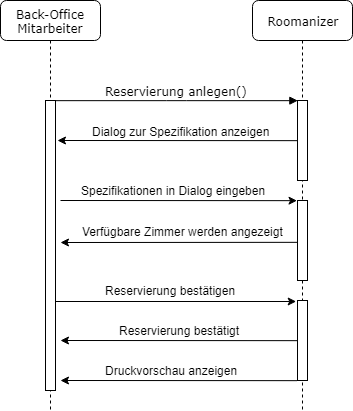
\includegraphics[width=0.7\linewidth]{./content/usecases/UseCase_ReservierungIndividualgastSequenze.png}
    \subsubsection{Kontrakte}
\end{document}